\documentclass[]{scrartcl}
\usepackage{Preamble}

\setcounter{section}{4}
\newcommand{\exercise}{Exercise \thesection}
\newcommand{\duedate}{2020-12-14, 23:59}

\begin{document}
\section*{\exercise}

To compile: unzip our uploaded code, and run \verb|make| inside \verb|code/|.
The slurm scripts are stored inside \verb|code/slurm/|.
To debug: run the debug outputs (\verb|*.dbg|) and attach gdb to respective pids

\subsection{Reading}

The Paper \enquote{The Future of Microprocessors} by Shekhar Borkar and Andrew Chien
describes the end of performance scaling via transistor-speed of microprocessors.
Instead, according to the authors, massive changes in architecture are necessary to keep
up with Moore's Law. The main reason for this is energy efficiency which will become the
key metric in chip design.
By simply adding as many compute cores at maximum frequency as the transistor-integration
capacity allows for the power consumption of the microprocessor would quickly grow into
the hundreds of Watts.
Instead of more fully fletched compute cores the authors suggest that instead both
cache size will grow further since caches require less energy compared to logic
and that microprocessors will instead feature smaller fine grained compute cores
capable of operating at different frequencies or accelerators for special workloads.

Some of the predictions made in the paper held true.
For example frequency adjustment for certain cores is common even in consumer grade CPUs
(Intel Turbo Boost, AMD Turbo Core).
On the other hand cache sizes did not grow as rapidly as predicted. Most off the shelf CPUs
feature caches in the range of \SI{30}{\mega B} with some going as high as \SI{64}{\mega B}.
Exceptions to this are exotic architectures like the \emph{IBM z15} that feature very large
off-chip caches realised as eDRAMs (\SI{960}{\mega B} L4 cache).
Also the incorporation of smaller compute cores and accelerators into the CPU is
mostly only found in exotic architectures. x64 based systems seem to stick to
external many core accelerators like \emph{GPUs} or the \emph{Xeon Phi}.
Despite that the core premise of the paper held true as energy efficiency has become
a very important metric not only in HPC but also in consumer grade computing
especially mobile devices.
We therefore accept the paper.

\subsection{Matrix multiply --- parallel version using MPI}\label{ssec:mmul_parallel}
\subsection{Matrix multiply --- scaling process count}\label{ssec:mmul_proc}

The program of \autoref{ssec:mmul_parallel} was tested on its scalability with an increasing number of processes.
The times and speedups in \autoref{tab:proc} were observed for 2000x2000 matrices with 100 repetitions.

\begin{table}[ht]
    \centering
    \begin{tabular}{rr}
\toprule
 nodes &  GFLOPS64/s \\
\midrule
     1 &     1.55161 \\
     3 &     2.28341 \\
     5 &     2.89719 \\
     7 &     3.89113 \\
     9 &     4.90389 \\
    11 &     5.42166 \\
    13 &     6.30550 \\
    15 &     7.30316 \\
\bottomrule
\end{tabular}

    \caption{Scaling by Processes in numbers}\label{tab:proc}
\end{table}

For this Example a step is visible before 6 pocesses, most likeley because here only one node is used and we are reaching its maximum. Starting with 6 processes, this maximum is increased.

\begin{figure}[H]
    \centering
    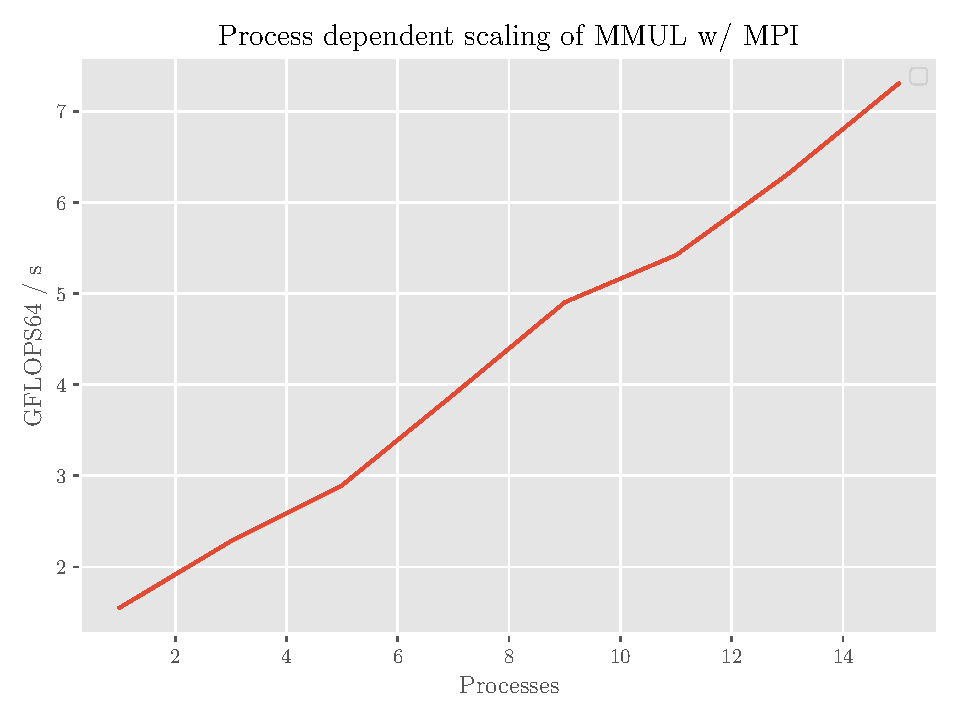
\includegraphics[width=\linewidth]{img/scaling_proc.pdf}
    \caption{Scaling Process Count}%
    \label{fig:scaling_proc}
\end{figure}

\subsection{Matrix multiply --- scaling problem size}
In addition to the process scaling in \autoref{ssec:mmul_proc}, the scaling by problem size was also observed. The observed numbers are shown in \autoref{tab:prob}, here each test was run for both 10 and 16 processes as well as repeated 10 times.

\begin{table}[ht]
    \centering
    \begin{tabular}{llrr}
\toprule
     &    & \multicolumn{2}{l}{GFLOPS64/s} \\
     &    &       mean &    std \\
dim & nodes &            &        \\
\midrule
128  & 10 &      0.778 &  0.058 \\
     & 16 &      0.407 &  0.012 \\
256  & 10 &      3.056 &  0.249 \\
     & 16 &      2.523 &  0.106 \\
512  & 10 &      5.164 &  0.204 \\
     & 16 &      6.505 &  1.947 \\
1024 & 10 &      4.529 &  0.687 \\
     & 16 &      3.231 &  1.393 \\
2048 & 10 &      5.281 &  0.132 \\
     & 16 &      7.451 &  0.967 \\
4096 & 10 &      5.593 &  0.054 \\
     & 16 &      8.601 &  0.128 \\
\bottomrule
\end{tabular}

    \caption{Scaling by Problem Size in numbers}\label{tab:prob}
\end{table}
\begin{figure}[H]
    \centering
    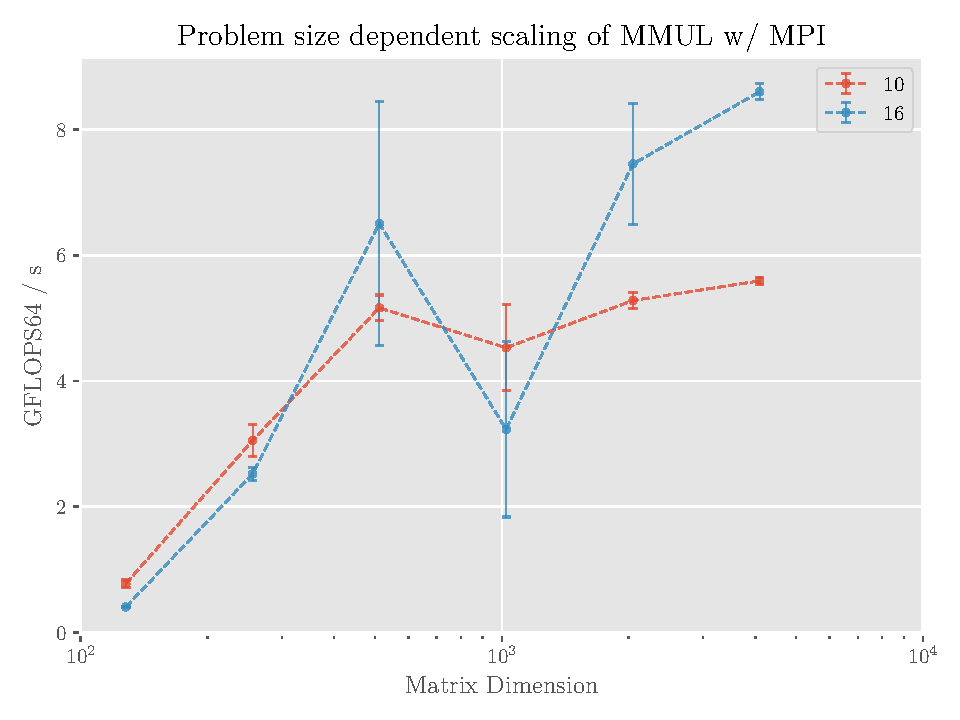
\includegraphics[width=\linewidth]{img/scaling_prob.pdf}
    \caption{Scaling Problem Size}%
    \label{fig:scaling_prob}
\end{figure}

\end{document}
